\documentclass[../main.tex]{subfiles}
\begin{document}
\section{里程估计}
\subsection{里程估计的基本概念}
\begin{enumerate}
    \item \textbf{里程估计(Odometry Estimation)}:根据\textbf{传感器感知信息}推导机器人\textbf{位姿}(位置和角度)变化\footnote{目的是进行航位推算(Dead-reckoning):基于已知位置,利用里程估计推算当前位置。}\\
    \begin{small}\kaishu
    Q:为什么不使用发送给机器人的运动控制指令进行航位推算?
    \\
    A:由于控制系统存在\textbf{滞后性(latency)}和可能的\textbf{超调(overshoot)},机器人\textbf{实际执行的控制指令}与\textbf{发送的控制指令}往往存在偏差。 \footnote{最早的里程估计方法即是根据码盘测得的实际速度进行位姿变化估计。}  
    \end{small}

    \item \textbf{基本思路*}:里程估计通过对机器人运动学模型进行积分,结合传感器提供的线速度与角速度,计算出机器人在连续时刻间的位姿变化。
    \begin{figure}[H]
        \centering
        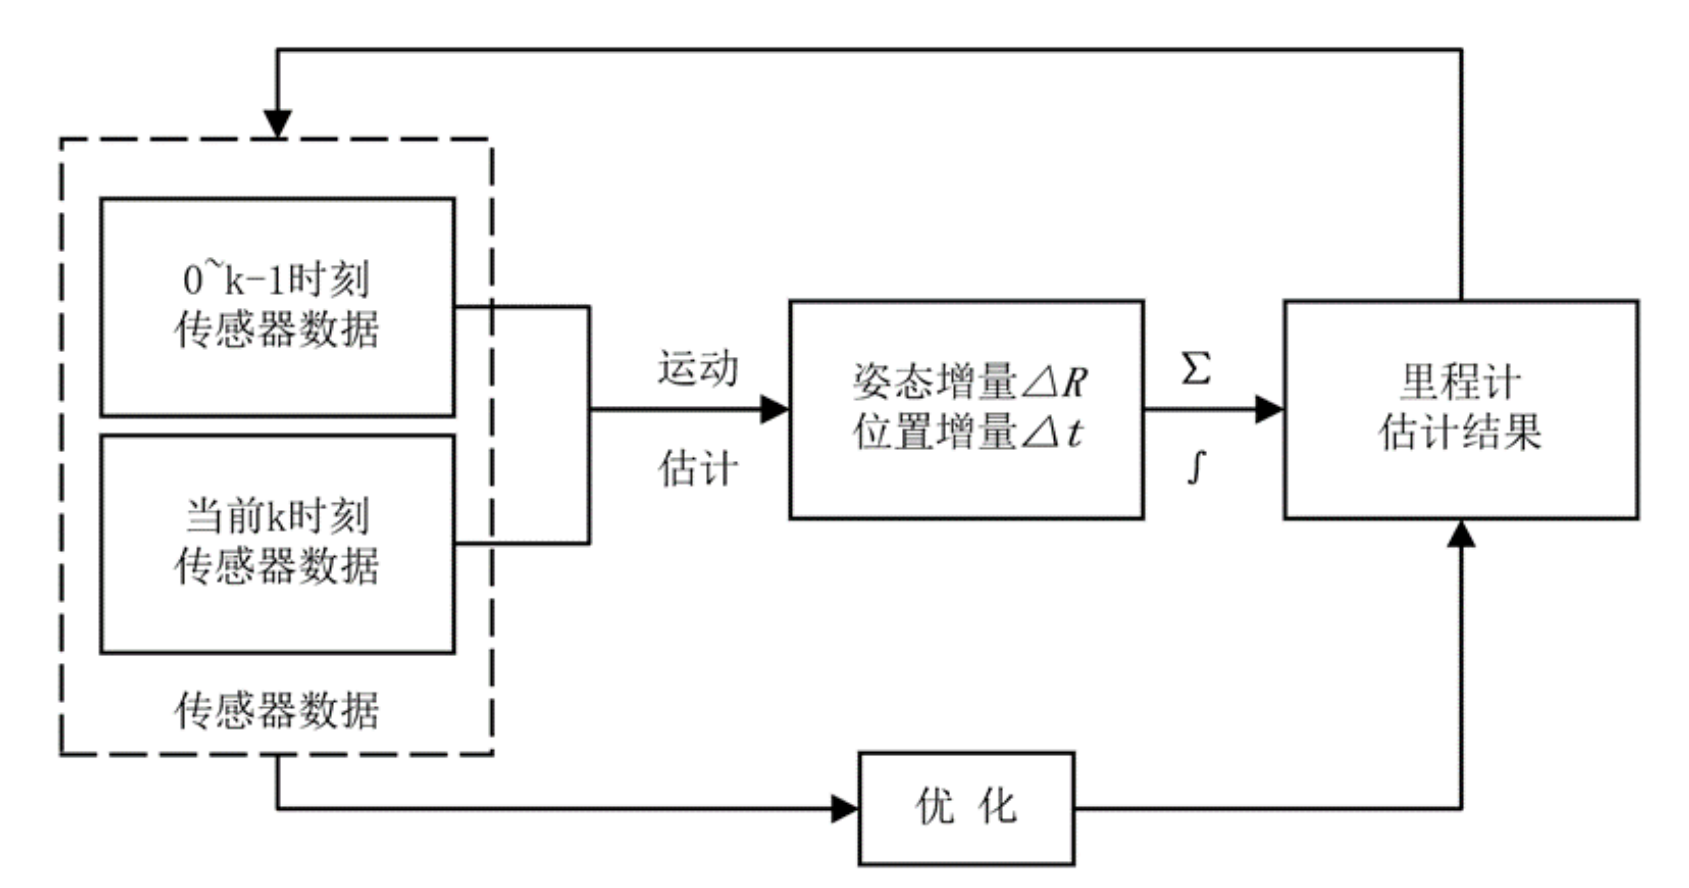
\includegraphics[width=0.7\textwidth]{images/odom.png}
        \caption{里程估计的基本思路}
    \end{figure}
    \item \textbf{主要方法}
    \begin{itemize}
        \item 基于\textbf{机器人运动感知信息}结合\textbf{运动学模型}:
        \begin{itemize}
            \item \hyperref[mapan]{电机码盘}(\textbf{轮式里程计})
            \item \hyperref[imu]{IMU}(惯性单元,加速度计 + 陀螺仪)(\textbf{惯性里程计})
        \end{itemize}
        \item 基于\textbf{环境感知传感器信息},通过\textbf{最优匹配估计}:
        \begin{itemize}
            \item \hyperref[laser]{激光里程计}(\textbf{Laser Odometry, LO})
            \item \hyperref[visual]{视觉里程计}(\textbf{Visual Odometry, VO})
        \end{itemize}
    \end{itemize}

    \item \textbf{位姿变化的数学描述}
    \begin{itemize}
        \item 二维平面运动: \((\Delta x, \Delta y, \Delta \theta)\)
        \item 三维空间运动: \((\Delta x, \Delta y, \Delta z, \Delta \alpha, \Delta \beta, \Delta \gamma)\)
        \item 一般统一表示为旋转矩阵与平移向量:
        \[
        R =
        \begin{bmatrix}
            r_{11} & r_{12} & r_{13} \\
            r_{21} & r_{22} & r_{23} \\
            r_{31} & r_{32} & r_{33}
        \end{bmatrix}
        \quad
        t = [\Delta x, \Delta y, \Delta z]^T,
        \]
        \\则有位姿变化:
        \[
        x' = R x + t,
        \]
    \end{itemize}
    \item \textbf{旋转矩阵与姿态变化关系}
    \begin{itemize}
        \item 绕 $x$ 轴旋转(\textbf{roll, 横滚角}):
        \[
        R_x =
        \begin{bmatrix}
            1 & 0 & 0 \\
            0 & \cos\theta & -\sin\theta \\
            0 & \sin\theta & \cos\theta
        \end{bmatrix}
        \]
        \item 绕 $y$ 轴旋转(\textbf{pitch, 俯仰角}):
        \[
        R_y =
        \begin{bmatrix}
            \cos\theta & 0 & \sin\theta \\
            0 & 1 & 0 \\
            -\sin\theta & 0 & \cos\theta
        \end{bmatrix}
        \]
        \item 绕 $z$ 轴旋转(\textbf{yaw, 偏航角}):
        \[
        R_z =
        \begin{bmatrix}
            \cos\theta & -\sin\theta & 0 \\
            \sin\theta & \cos\theta & 0 \\
            0 & 0 & 1
        \end{bmatrix}
        \]
        \item 组合旋转:  
        \[
        R = R_z(\Delta\gamma) R_y(\Delta\beta) R_x(\Delta\alpha)
        \]
    \end{itemize}

    \item \textbf{由旋转矩阵求欧拉角}
    \begin{itemize}
        \item 当旋转矩阵为
        \[
        R = 
        \begin{bmatrix}
            r_{11} & r_{12} & r_{13} \\
            r_{21} & r_{22} & r_{23} \\
            r_{31} & r_{32} & r_{33}
        \end{bmatrix},
        \]
        根据分解关系有:
        \[
        \Delta\alpha = \mathrm{atan2}(r_{32}, r_{33}), \quad
        \Delta\beta = \mathrm{atan2}(-r_{31}, \sqrt{r_{32}^2 + r_{33}^2}), \quad
        \Delta\gamma = \mathrm{atan2}(r_{21}, r_{11})
        \]
        \item {欧拉角表示具有几何直观性,但存在奇异性问题:当俯仰角 $\pm 90^\circ$ 时,产生万向锁问题。}
    \end{itemize}

    \item \textbf{四元数表示法}
    \begin{itemize}
        \item 在实际应用中,常采用四元数(Quaternion)来表示旋转\footnote{利用四元数可避免对旋转欧拉角的解算,直接进行旋转变换}。
        \item 三维空间的任意旋转可表示为绕单位旋转轴 $\mathbf{n} = (n_x, n_y, n_z)$ 旋转角度 $\theta$:
        \[
        (\theta, n_x, n_y, n_z)^T
        \]
        \item 四元数定义:
        \[
        q = (q_0, q_1, q_2, q_3)^T = 
        (\cos\frac{\theta}{2}, n_x\sin\frac{\theta}{2}, n_y\sin\frac{\theta}{2}, n_z\sin\frac{\theta}{2})^T
        \]
        \item 三维空间点表示为虚四元数:
        \[
        p = (0, x, y, z)
        \]
        \item 旋转后的点:
        \[
        p' = q p q^{-1}
        \]
        \item 四元数的代数运算规则:
        \[
        i^2 = j^2 = k^2 = -1,\quad
        ij = k, \ ji = -k,\quad
        jk = i, \ kj = -i,\quad
        ki = j, \ ik = -j
        \]
        \item 四元数对应的旋转矩阵:
        \[
        R = \begin{bmatrix}
            1 - 2q_2^2 - 2q_3^2 & 2q_1q_2 + 2q_0q_3 & 2q_1q_3 - 2q_0q_2 \\
            2q_1q_2 - 2q_0q_3 & 1 - 2q_1^2 - 2q_3^2 & 2q_2q_3 + 2q_0q_1 \\
            2q_1q_3 + 2q_0q_2 & 2q_2q_3 - 2q_0q_1 & 1 - 2q_1^2 - 2q_2^2
        \end{bmatrix}
        \]
        \item 由旋转矩阵求解四元数(当 $q_0 \neq 0$ 且 $1 + r_{11} + r_{22} + r_{33} > 0$):
        \[
        q_0 = \frac{\sqrt{\mathrm{tr}(R) + 1}}{2}, \quad
        q_1 = \frac{r_{23} - r_{32}}{4q_0}, \quad
        q_2 = \frac{r_{31} - r_{13}}{4q_0}, \quad
        q_3 = \frac{r_{12} - r_{21}}{4q_0}
        \]
        \item 四元数的优点:
        \begin{itemize}
            \item 表达更紧凑;
            \item 求解无奇异
            \item 计算更快速
        \end{itemize}
    \end{itemize}

\end{enumerate}

\subsection{基于运动感知的里程估计}
\begin{enumerate}
    \item \textbf{基于电机码盘的轮式移动机器人里程估计}\label{mapan}
        \begin{itemize}
            \item \textbf{基本步骤}
            \begin{itemize}
                \item (1)根据电机码盘获得轮子转速  
                \[
                \dot{\varphi} = \frac{2\pi n}{\eta}
                \]
                其中:
                \begin{itemize}
                    \item \( n \):码盘测量得到的电机转速(转/分);
                    \item \( \eta \):齿轮减速比。
                \end{itemize}
                
                \item (2)结合运动学模型计算参考点速度  
                    \begin{figure}[H]
                        \centering
                        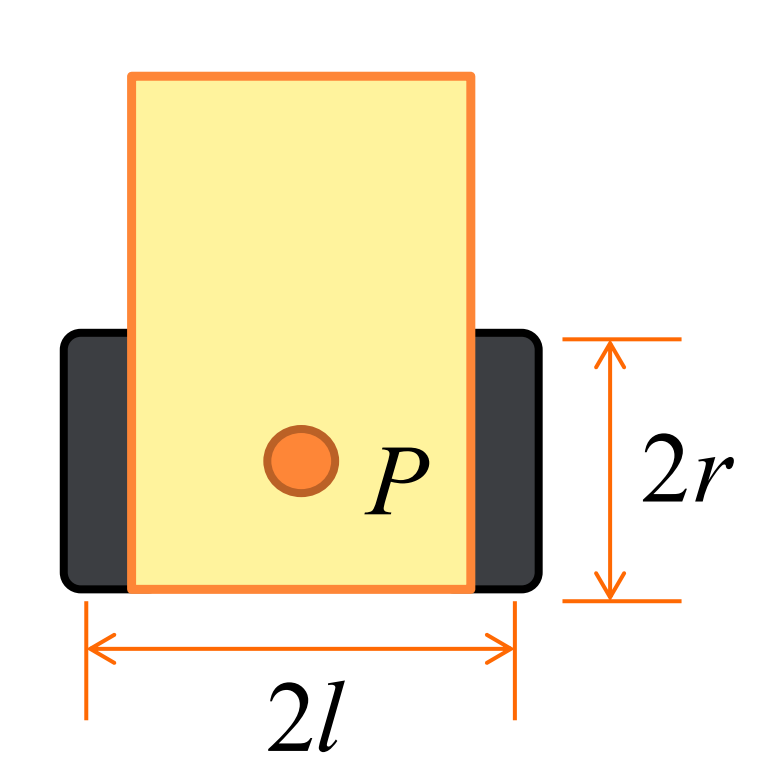
\includegraphics[width=0.2\textwidth]{images/smallcar.png}
                        \caption{差分驱动机器人示例}
                    \end{figure}
                对于差动驱动机器人(两轮间距为 $2l$,轮半径为 $r$):
                
                \[
                v = \frac{r \dot{\varphi}_l}{2} + \frac{r \dot{\varphi}_r}{2}, \quad
                \omega = \frac{r \dot{\varphi}_l}{2l} - \frac{r \dot{\varphi}_r}{2l}
                \]
                
                \item (3)假设短时间片内为匀速运动,计算位姿变化:
                \[
                \Delta d = v \Delta t, \quad \Delta \theta = \omega \Delta t
                \]

                \item (4)基于位姿变化的航位推算
                \begin{itemize}
                    \item 当已知时刻 \(t-1\) 的位姿 \(x_{t-1} = (x_{t-1}, y_{t-1}, \theta_{t-1})^T\),根据上一时间步的里程增量 \((\Delta d, \Delta \theta)\),可得下一时刻 \(t\) 的位姿:
                    \[
                    \begin{cases}
                    x_t = x_{t-1} + \Delta d \cos(\theta_{t-1} + \Delta\theta) \\
                    y_t = y_{t-1} + \Delta d \sin(\theta_{t-1} + \Delta\theta) \\
                    \theta_t = \theta_{t-1} + \Delta\theta
                    \end{cases}
                    \]
                \end{itemize}
            \end{itemize}
    
            \item \textbf{轮式里程估计误差}
            \begin{itemize}
                \item \textbf{系统误差(Systematic Errors)}
                \begin{itemize}
                    \item 轮半径误差;
                    \item 轮子安装精度误差(不平行、两边距离不相等);
                    \item 编码器精度误差;
                    \item 采样精度误差;
                    \item 齿轮减速比精度。
                \end{itemize}
    
                \item \textbf{偶然误差(Random Errors)}
                \begin{itemize}
                    \item 地面不平;
                    \item 轮子打滑;
                \end{itemize}
    
                \item \textbf{里程计误差导致的问题}
                \begin{itemize}
                    \item 在航位推算时,里程计误差被\textbf{累加}                    \footnote{即便每次误差极小,积累后也会导致轨迹与实际路径产生显著偏离。};
                    \item \textbf{推算误差随时间增长而不断扩大};
                    \item 公式描述如下:
                    \[
                    \begin{cases}
                    x_t = x_{t-1} + \Delta d \cos(\theta_{t-1} + \Delta\theta) \\
                    y_t = y_{t-1} + \Delta d \sin(\theta_{t-1} + \Delta\theta) \\
                    \theta_t = \theta_{t-1} + \Delta\theta
                    \end{cases}
                    \]

                \end{itemize}
            \end{itemize}
        \end{itemize}
    \item \textbf{基于惯性单元的里程估计}\label{imu}
        \begin{itemize}
            \item \textbf{组成}:一般含有三轴的加速度计和三轴的陀螺仪;通常集成一个三轴磁力计用于校正 IMU 的姿态估计通过积分运算可得载体在导航坐标系中的姿态、速度和位置等信息
            \item \textbf{原理}:通过\textbf{积分运算}可得载体在导航坐标系中的姿态、速度和位置等信息
            \item \textbf{优点}:
                \begin{itemize}
                    \item 全天候
                    \item 采样频率高
                    \item 短时精度较好
                \end{itemize}
            \item \textbf{缺点}:
                \begin{itemize}
                    \item 误差累积:随着时间的增长累积误差较大,无法满足移动机器人长距
离精确定位的要求,需要融合其它传感器进行组合导航
                \end{itemize}
        \end{itemize}

\end{enumerate}
\subsection{基于环境感知的里程估计}
\begin{enumerate}
\item \textbf{激光里程计(ICP算法)}\label{laser}
                    \begin{figure}[H]
                        \centering
                        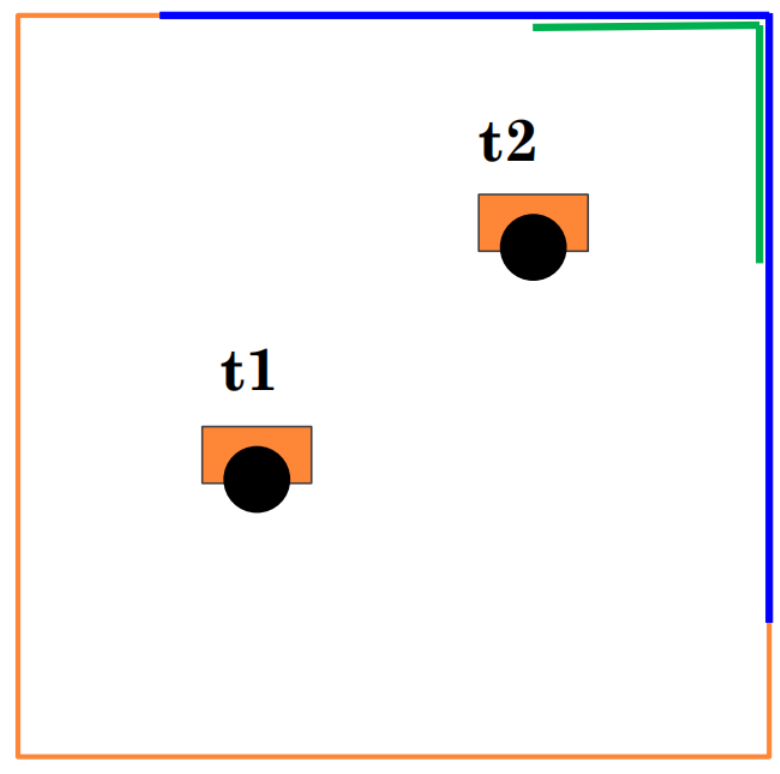
\includegraphics[width=0.3\textwidth]{images/laser.png}
                        \caption{LO场景示例}
                    \end{figure}
    \begin{itemize}
        \item \textbf{基本步骤}:
        \begin{enumerate}
            \item 估计 $P'$ 集合点与 $P$ 集合点的初始位姿关系;
            \item 根据最近邻域规则建立 $P'$ 集合点与 $P$ 集合点的关联;
            \item 利用线性代数 / 非线性优化的方式估计旋转平移量;
            \item 对点集合 $P'$ 的点进行旋转平移;
            \item 如果旋转平移后重新关联的均方差小于阈值,则结束;
            \item 否则迭代重复上述步骤。
        \end{enumerate}

        \item \textbf{ICP类别}:
        \begin{itemize}
            \item Point to Point
            \item Line to Line
            \item Plane to Plane
            \item Point to Line
            \item Point to Plane
            \item Line to Plane
        \end{itemize}

        \item \textbf{点对点ICP(Point-to-Point ICP)}\footnote{省流:运筹学最优化的问题,输入上一帧点集合和当前点集合的位置,构造目标函数使得两组点经R、t的一个变换后距离误差最小,寻找最优的R、t;先通过可能的IMU等等得到一个初值R、t,然后开始迭代求解}
        \begin{itemize}
            \item \textbf{输入:}  
            点集合 \( P, P' \),
            \[
            P = \{ \mathbf{p}_1, \dots, \mathbf{p}_n \}, \quad P' = \{ \mathbf{p}'_1, \dots, \mathbf{p}'_n \}
            \]

            \item \textbf{目标:}  
            计算两组数据之间的旋转平移量 \( R, t \),
            使得两组数据形成最佳匹配,即两组点的距离误差最小。

            \item \textbf{构造目标函数:}  
            第 \( i \) 个匹配点的误差为:
            \[
            \mathbf{e}_i = \mathbf{p}_i - (R \mathbf{p}'_i + t)
            \]
            由此构建最小二乘问题:
            \[
            \min_{R, t} \frac{1}{2} \sum_{i=1}^{n} \left\| \mathbf{p}_i - (R \mathbf{p}'_i + t) \right\|^2
            \]
            \begin{small}\kaishu
            \item \textbf{线性代数求解方法:}
            \begin{enumerate}
                \item 定义两组点集合的质心位置:
                \[
                \mathbf{p} = \frac{1}{n} \sum_{i=1}^{n} \mathbf{p}_i, \quad
                \mathbf{p}' = \frac{1}{n} \sum_{i=1}^{n} \mathbf{p}'_i
                \]
                \item 计算去质心坐标\footnote{去掉质心(即转到两组点的局部坐标系)可以让平移项$t$消失,从而将问题简化为只关于旋转$R$的最小化问题}:
                \[
                \mathbf{q}_i = \mathbf{p}_i - \mathbf{p}, \quad
                \mathbf{q}'_i = \mathbf{p}'_i - \mathbf{p}'
                \]
                \item 构建优化问题,计算旋转矩阵:
                \[
                R^* = \arg\min_R \frac{1}{2} \sum_{i=1}^{n} \left\| \mathbf{q}_i - R \mathbf{q}'_i \right\|^2
                \]
                \item 根据旋转矩阵 \( R \) 计算平移向量:
                \[
                t^* = \mathbf{p} - R \mathbf{p}'
                \]
            \end{enumerate}

            \item \textbf{R, t 分解计算说明:}
            \begin{align*}
                \frac{1}{2}\sum_{i=1}^{n}\|\mathbf{p}_i - (R\mathbf{p}'_i + t)\|^2 
                &= \frac{1}{2}\sum_{i=1}^{n}\|(\mathbf{p}_i - \mathbf{p}) - R(\mathbf{p}'_i - \mathbf{p}')\|^2 
                + \|\mathbf{p} - R\mathbf{p}' - t\|^2
            \end{align*}
            优化目标函数可简化为:
            \[
            \min \frac{1}{2}\sum_{i=1}^{n}\|(\mathbf{p}_i - \mathbf{p}) - R(\mathbf{p}'_i - \mathbf{p}')\|^2 + \|\mathbf{p} - R\mathbf{p}' - t\|^2
            \]
            左项仅与旋转矩阵 \(R\) 相关,右项仅与质心相关,因此可分解为两步法求解。

            \item \textbf{求解旋转矩阵 \( R \):}
            \begin{align*}
            \min_R \frac{1}{2}\sum_{i=1}^{n}\|\mathbf{q}_i - R\mathbf{q}'_i\|^2
            &= \frac{1}{2}\sum_{i=1}^{n} \big( \mathbf{q}_i^T\mathbf{q}_i
                + (\mathbf{q}'_i)^T R^T R\,\mathbf{q}'_i
                - 2\mathbf{q}_i^T R\mathbf{q}'_i \big) \\
            &\Rightarrow \max_R \sum_{i=1}^{n} \mathbf{q}_i^T R \mathbf{q}'_i
            \end{align*}
            定义矩阵:
            \[
            W = \sum_{i=1}^{n} \mathbf{q}'_i \mathbf{q}_i^T
            \]
            对 \(W\) 进行 SVD 分解:
            \[
            W = U S V^T, \quad R = V U^T
            \]

            \item \textbf{求解平移向量 \( t \):}
            \[
            t = \mathbf{p} - R \mathbf{p}'
            \]

            \item \textbf{目标函数上界分析:}
            \[
            \text{tr}(RUSV^T) = \text{tr}(S^T R U) \sim \text{tr}(SH)
            \]
            其中 \(H = (h_1^T, h_2^T, h_3^T)^T\),\(h_i\) 为模长为 1 的向量,
            因此目标函数上界为:
            \[
            \text{tr}(RUSV^T) \le s_1 + s_2 + s_3
            \]
            当 \(H = V^T R U = I\) 时取等号,即:
            \[
            R = VU^T
            \]
            并进一步得到:
            \[
            t = \mathbf{p} - R \mathbf{p}'
            \]
            \end{small}
        \end{itemize}

        \item \textbf{关于ICP的思考}
        \begin{itemize}
            \item \textbf{Q: ICP计算效率主要受什么影响?} \\
            \textbf{A:} 主要受\textbf{最近邻点搜索}\footnote{让当前点云中每个点都去找在目标点云中最近的一个点作为配对点}影响。每次迭代都需要在目标点云中为源点寻找最近点,若使用暴力搜索,复杂度为 $O(N^2)$\footnote{实际中常使用 KD-Tree、Octree 或体素网格(Voxel Grid)结构加速最近邻匹配,从而显著提升计算效率。}。

        
            \item \textbf{Q: ICP迭代寻优会存在什么问题?} \\
            \textbf{A:} 主要存在\textbf{局部最优}问题。由于ICP基于最小二乘匹配,若初始位姿估计较差,点云可能收敛到错误的局部极值位置;此外,当重叠区域过小或噪声较大时,算法稳定性下降、收敛速度变慢。
        
            \item \textbf{Q: 对于移动机器人来讲,两帧点云数据做ICP的初值如何获得?} \\
            \textbf{A:} 初始位姿可由\textbf{里程计(Odometry)}、\textbf{IMU惯性测量单元}、或\textbf{上一帧的位姿估计结果}提供。  
            这些先验信息可作为ICP的初值输入,使迭代更快收敛并避免陷入局部最优。
        \end{itemize}
    \end{itemize}
    \item \textbf{视觉里程计}\label{visual}
        \begin{itemize}
            \item \textbf{原理}:检测由运动所导致的图像变化来估计两帧数据之间的位姿变化量
                    \begin{figure}[H]
                        \centering
                        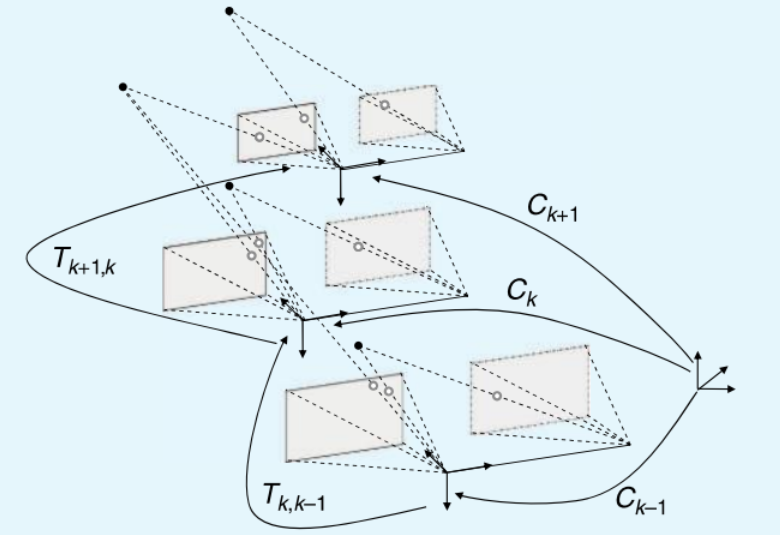
\includegraphics[width=0.4\textwidth]{images/vo.png}
                        \caption{VO场景示例}
                    \end{figure}
            \item \textbf{分类}
                \begin{itemize}
                    \item \textbf{基于图像的VO}:利用两幅图像中\textbf{所有}像素的\textbf{亮度}信息——计算量大、精确度低
                    \item \textbf{基于特征的VO}:从图像中提取醒目的\textbf{可重复的特征}——要求两帧之间鲁棒匹配或者跟踪特征
                \end{itemize}
            \item \textbf{优点}
                \begin{itemize}
                    \item 可以避免里程估计受地面不平整的影响
                \end{itemize}
            \item \textbf{缺点}
                \begin{itemize}
                    \item 应用对环境有多方面要求
                        \begin{enumerate}
                            \item 环境光照足够
                            \item 场景包含足够纹理
                            \item 相邻帧之间有足够的重叠内容
                            \item 场景静态
                        \end{enumerate}
                    \item 噪声和错误匹配仍会影响里程估计的准确性,并会被不断叠加
                \end{itemize}            
            \item \textbf{基于特征的VO具体步骤}
                    \begin{figure}[H]
                        \centering
                        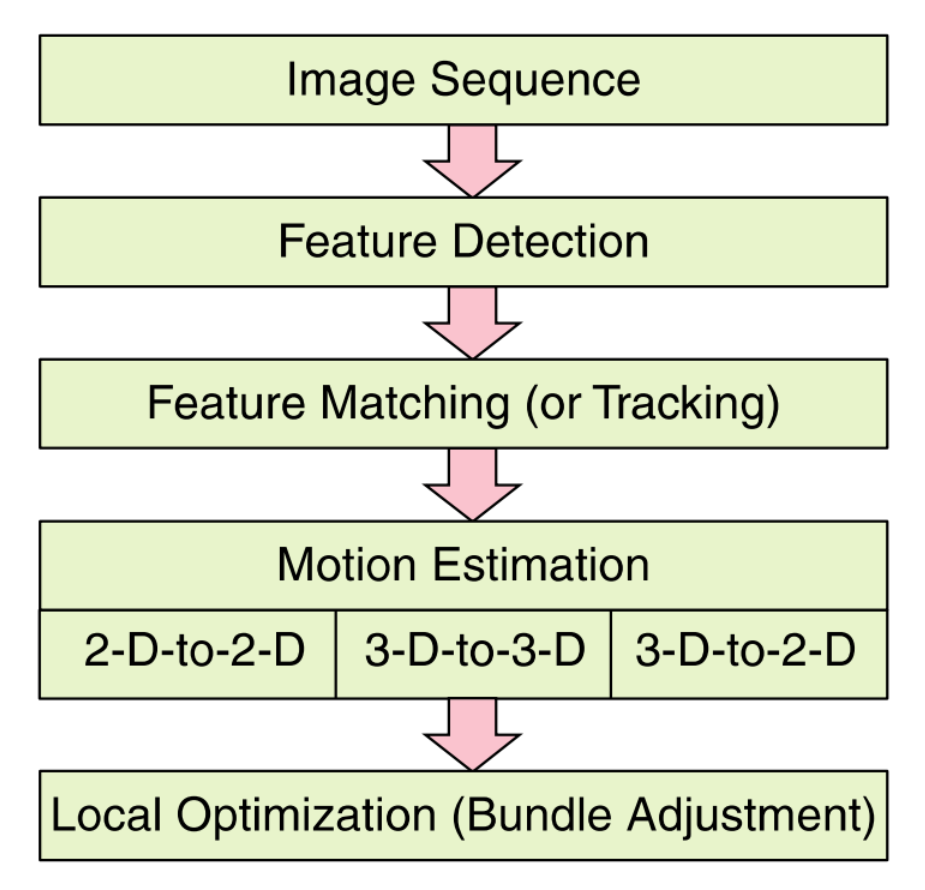
\includegraphics[width=0.4\textwidth]{images/vo_structure.png}
                        \caption{基于特征的VO求解框架}
                    \end{figure}
                \begin{enumerate}
                    \item \textbf{Step1:特征检测}
                        \begin{itemize}
                            \item \textbf{特征的基本概念}:
                                \begin{enumerate}
                                    \item \textbf{图像特征的概念}:图像中有代表性的点
                                    \item \textbf{图像特征的例子}:
                                        \begin{itemize}
                                            \item \textbf{角点特征(corner)}:ORB, Haris, Shi-Tomasi, FAST
                                            \item \textbf{圆块特征(blob)}:SIFT, SURF, CENSURE
                                        \end{itemize}
                                    \item \textbf{特征点描述}:
                                    \begin{itemize}
                                        \item \textbf{关键点(Key-point)}:描述特征在图像中的\textbf{位置}等信息
                                        \item \textbf{描述子(Descriptor)}:描述该关键点与\textbf{邻域}在\textbf{亮度、颜色、纹理}等方面的图像模式
                                    \end{itemize}
                                    \item \textbf{特征特性}:可重复性\footnote{即大量特征应在下一幅图像中出现}、不变性\footnote{光照不变性、几何不变性(旋转、尺度、视点)}、独特性、鲁棒性\footnote{适应噪声、压缩、模糊}、定位准确性\footnote{包括位置和尺度}、计算效率高
                                \end{enumerate}
                            \item \textbf{ORB特征}:
                                                \begin{figure}[H]
                                                    \centering
                                                    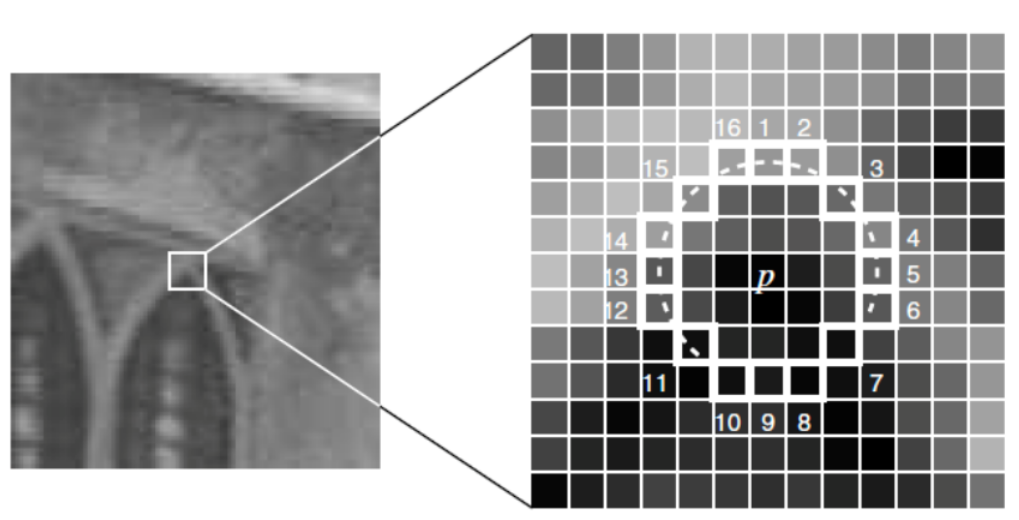
\includegraphics[width=0.5\textwidth]{images/orb1.png}
                                                    \caption{Oriented FAST}
                                                \end{figure}
                                \begin{itemize}
                                    \item \textbf{关键点}:\textbf{Oriented FAST} 
                                        \begin{itemize}
                                            \item \textbf{角点}\footnote{角点(corner) 是一种特定类型的特征点(feature point);而关键点(keypoint) 是在角点基础上进一步赋予了尺度、方向等属性的“可匹配特征点”。}:局部像素灰度变化明显的像素。
                                            \item \textbf{角点获取方法}:
                                                \begin{figure}[H]
                                                    \centering
                                                    % --- 左图 ---
                                                    \begin{minipage}[t]{0.35\textwidth}
                                                        \centering
                                                        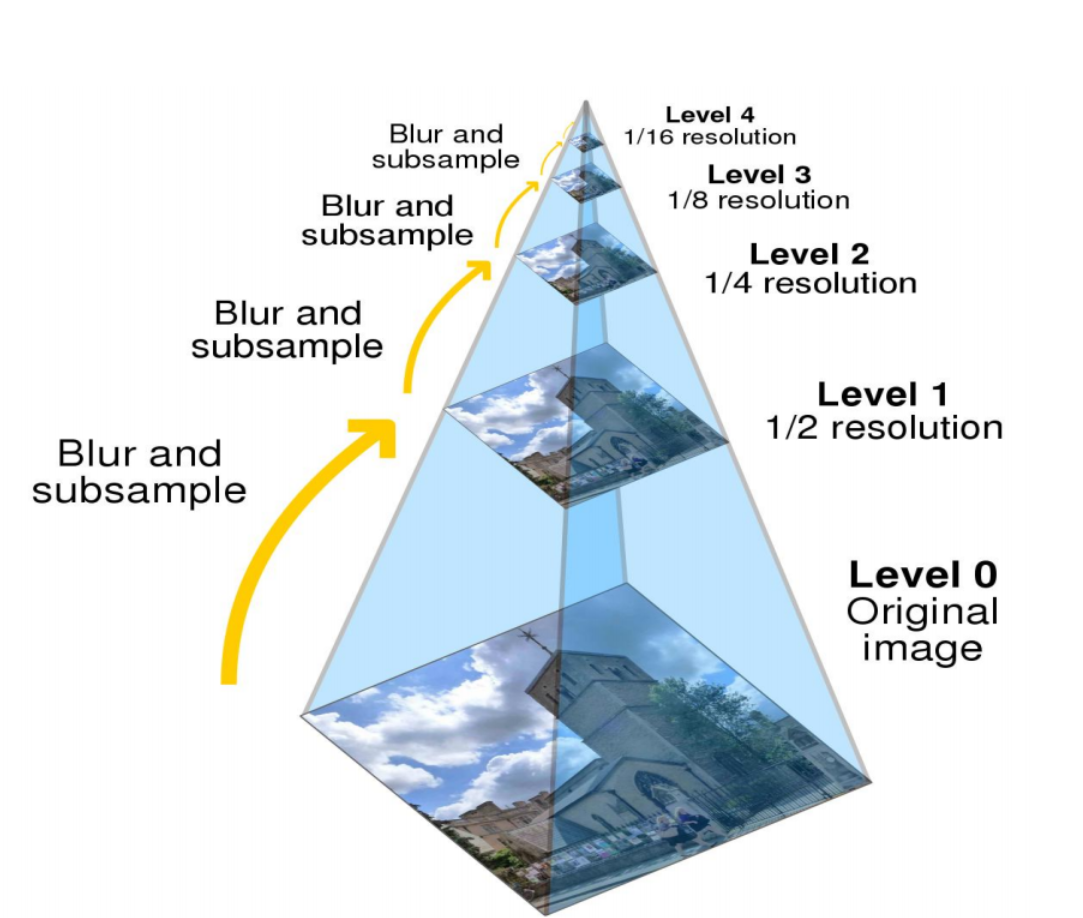
\includegraphics[width=\textwidth]{images/orb2.png}
                                                        \caption{图像金字塔}
                                                        \label{fig:orb_pyramid}
                                                    \end{minipage}
                                                    % --- 右图 ---
                                                    \begin{minipage}[t]{0.35\textwidth}
                                                        \centering
                                                        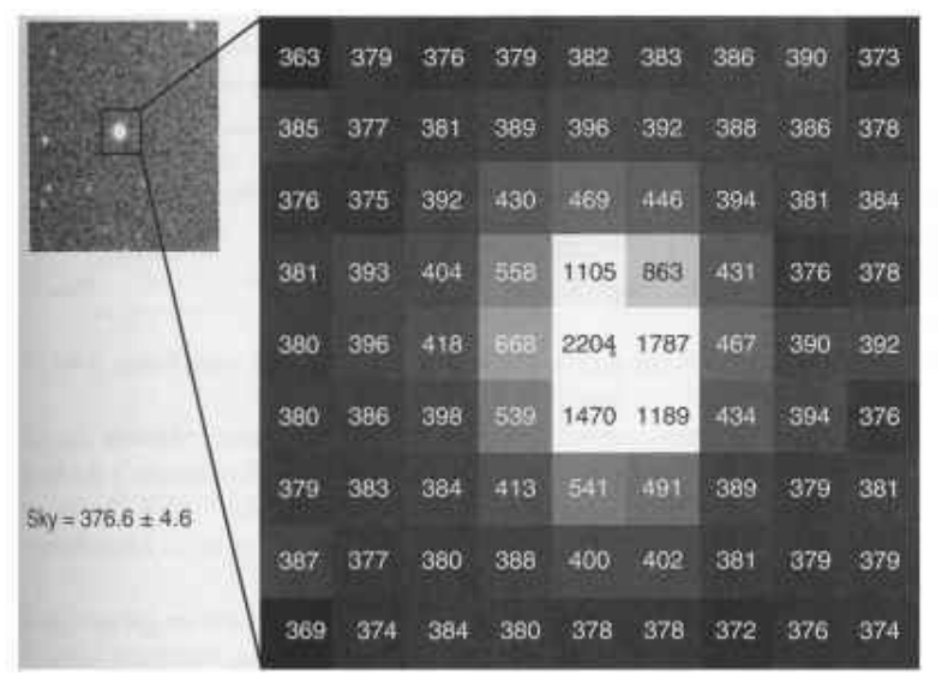
\includegraphics[width=\textwidth]{images/orb3.png}
                                                        \caption{灰度质心法}
                                                        \label{fig:orb_centroid}
                                                    \end{minipage}
                                                \end{figure}
                                                \textbf{FAST}:Features from Accelerated Segment Test,以像素点为中心一定半径的圆上,有连续N个点与像素灰度值差大于阈值
                                                \textbf{Oriented FAST}:FAST的优化,通过构建\textbf{图像金字塔}\footnote{在不同尺度(图像大小)下都能检测到稳定的特征点,将原始图像逐层下采样,形成多层图像,使物体在图像中变大或变小,检测出的关键点位置仍然一致。}和\textbf{灰度质心法}\footnote{它通过计算角点邻域的灰度质心(intensity centroid)来求出主方向角,根据灰度值总和与坐标-灰度值乘积总和计算质心坐标。无论图像如何旋转,ORB都会调整描述子的方向,使得特征点的描述结果保持一致}使特征具有\textbf{尺度不变性和旋转不变性}

                                        \end{itemize}
                                    \item \textbf{描述子}:\textbf{BRIEF} (Binary Robust Independent Elementary Feature)
                                        \begin{itemize}
                                            \item 通过0和1编码关键点附近两个像素的大小关系,对于像素p和q, 如果p比q大,则取1,反之取0
                                            \item 按概率分布生成随机取128个这样两个像素的模版,得到128维由0和1组成的向量
                                        \end{itemize}
                                \end{itemize}
                            
                    \item \textbf{Step2:特征匹配}
                        \begin{enumerate}
                            \item \textbf{暴力搜索}:(耗时,是\textbf{特征数的二次方})
                                \begin{enumerate}
                                    \item \textbf{单向匹配}:将第一帧图像中的所有特征与第二帧图像中的所有特征进行比较,相似度在阈值范围内的\textbf{建立对应关系}
                                    \item \textbf{反向匹配}:由于第一帧图像中的特征可能在第二帧图像中找到多个对应,因此需要进行\textbf{交叉一致性验证},即第二帧图像中的所有特征与第一帧图像中的所有特征进行比较,建立对应关系,当彼此相互存在对应关系时才认为匹配
                                \end{enumerate}
                            \item \textbf{增加约束条件}:核心目的是限制搜索区域\\
                            \noindent\textbullet\quad{区域约束}:根据运动预测
                                \begin{itemize}
                                    \item \textbf{特征点}:需要具备\textbf{三维空间位置}信息;
                                    \item \textbf{适用性}:适用于\textbf{运动偏移量较小、图像变化较小}的情况;
                                    \item 若要在\textbf{长图像序列}上采用跟踪策略,则需对每个特征建立\textbf{仿射变形模型}\footnote{以描述随时间的尺度、旋转和视角变化};
                                \end{itemize}
                            \noindent\textbullet\quad \textbf{极线约束}:根据立体视觉
                                \begin{itemize}
                                    \item \textbf{特征点}:\textcolor{red}{不}需要具备\textbf{三维空间位置}信息,特征非三维。
                                    \item \textbf{适用性}:适用于\textbf{运动偏移量较小、图像变化较小}的情况;
                                \end{itemize}
                                                \begin{figure}[H]
                                                    \centering
                                                    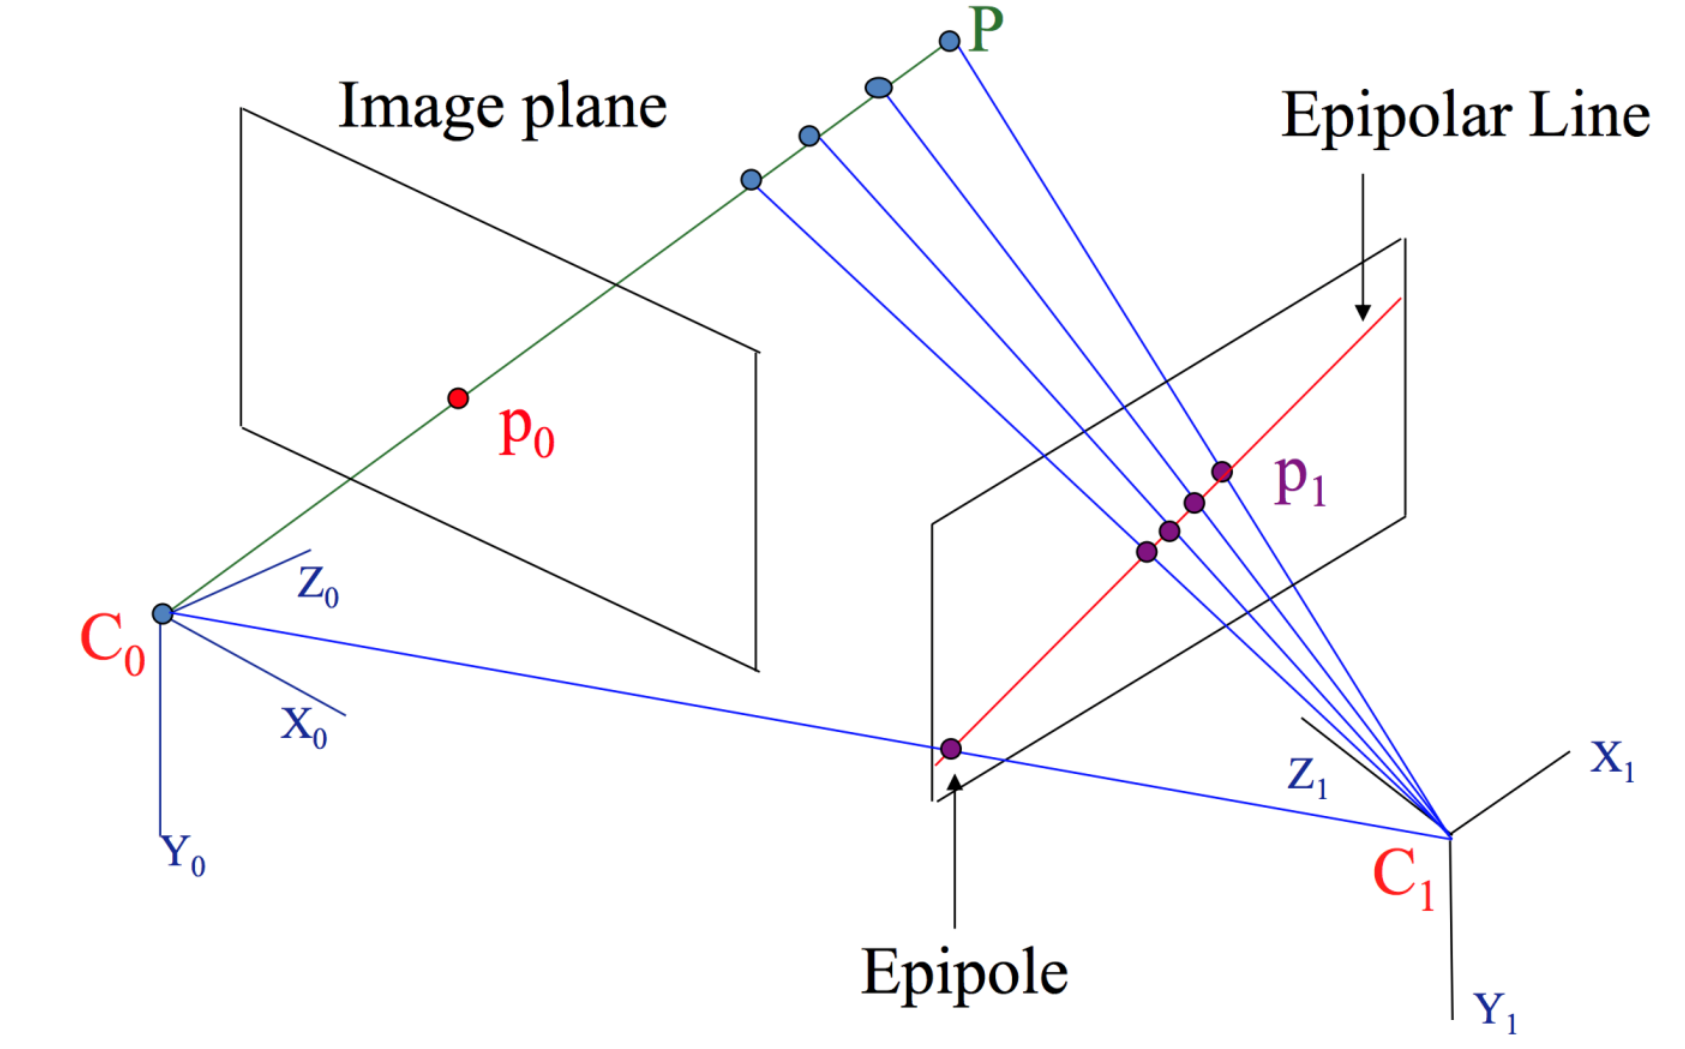
\includegraphics[width=0.5\textwidth]{images/jixian.png}
                                                    \caption{立体视觉}
                                                \end{figure}
                        \end{enumerate}
                    \item \textbf{Step3:运动估计} 
    \begin{itemize}
        \item \textbf{基本思路}:通过\textbf{两帧或多帧图像中的特征点匹配关系},估计相机在不同时间的\textbf{位姿变化(R, t)}\footnote{这一部分是整个视觉里程计与SLAM系统中“从特征匹配过渡到几何估计”的核心环节,是视觉运动估计的基础。}

        \item \textbf{根据相机类型的分类方法}:
\begin{enumerate} \item \textbf{单目相机(Monocular Camera)} \begin{itemize} \item 仅有\textbf{2D像素坐标}; \item 根据两组2D点的对应关系估计相机运动,属于\textbf{2D-to-2D}问题; \item 方法:\textbf{对极几何(Epipolar Geometry)}方法。 \end{itemize} \item \textbf{双目 / RGB-D 相机(Stereo or RGB-D Camera)} \begin{itemize} \item 每个像素都具有\textbf{距离信息}; \item 根据两组3D点估计相机运动,属于\textbf{3D-to-3D}问题; \item 方法:\textbf{ICP}方法。 \end{itemize} \item \textbf{具有三维点及其投影位置的相机(PnP Problem)} \begin{itemize} \item \textbf{3D-to-2D}关系; \item 方法:PnP方法。 \end{itemize} \end{enumerate}


        \item \textbf{2D-to-2D:对极几何}
        \\接下来对于这种情况,我们先给出一些前置的公式基础推导,之后在此基础上说明运动估计的求解步骤。
        \begin{itemize}
            \item \textbf{公式基础}:
                \begin{enumerate}
                    \item 相机模型:针孔模型下,有归一化坐标
                    \[
                    x_1 = K^{-1} \tilde{p}, \quad x_2 = K^{-1} p,
                    \]
                    其中 $K$ 为相机内参矩阵。
                    \item 对极约束公式如下,
                    \[
                    x_1^T E x_2 = 0, \quad \text{其中 } E = [t]_\times R.
                    \]
                    \item 本质矩阵 $E$ 与基础矩阵 $F$ 的关系为:
                    \[
                    F = K^{-T} E K^{-1}, \quad \text{对极约束 } p^T F \tilde{p} = 0.
                    \]
                    \footnote{几何意义:两相机中心与空间点形成的三角面称为“极平面”,极平面在两幅图像上与像平面交于“极线”,同一空间点的成像点必须分别位于对应极线上。}
            \end{enumerate}

            \item \textbf{运动估计的求解步骤}
            \begin{enumerate}
                \item 根据匹配点的像素坐标,计算基础矩阵 $F$ 或本质矩阵 $E$——\textbf{八点法};
                \item 根据 $E$ 或 $F$ 分解得到相机的旋转矩阵 $R$ 与平移向量 $t$——\textbf{SVD方法}\footnote{$E$ 与 $F$ 的区别仅在于是否包含相机内参,若内参已知,通常直接使用 $E$ 形式。}
            \end{enumerate}
        \end{itemize}
        \begin{small}\kaishu
        ==============================\\
        \item \textbf{本质矩阵的求解:八点法}
        \\$E$ 在不同尺度下等价,因此仅需8对匹配点即可求解——称为\textbf{八点法}
        \begin{itemize}
            \item 记一对匹配点的归一化坐标为:
            \[
            x_1 = [u_1, v_1, 1]^T, \quad x_2 = [u_2, v_2, 1]^T.
            \]
            \item 根据对极约束:
            \[
            (u_1, v_1, 1)
            \begin{bmatrix}
                e_1 & e_2 & e_3 \\
                e_4 & e_5 & e_6 \\
                e_7 & e_8 & e_9
            \end{bmatrix}
            (u_2, v_2, 1)^T = 0.
            \]
            \item 写成向量形式:
            \[
            [u_1u_2, u_1v_2, u_1, v_1u_2, v_1v_2, v_1, u_2, v_2, 1] \cdot e = 0,
            \]
            其中
            \[
            e = [e_1, e_2, e_3, e_4, e_5, e_6, e_7, e_8, e_9]^T.
            \]
            \item 由8对匹配点构造八点方程:
            \[
            \begin{bmatrix}
                u_1^1u_2^1 & u_1^1v_2^1 & u_1^1 & v_1^1u_2^1 & v_1^1v_2^1 & v_1^1 & u_2^1 & v_2^1 & 1 \\
                u_1^2u_2^2 & u_1^2v_2^2 & u_1^2 & v_1^2u_2^2 & v_1^2v_2^2 & v_1^2 & u_2^2 & v_2^2 & 1 \\
                \vdots & \vdots & \vdots & \vdots & \vdots & \vdots & \vdots & \vdots & \vdots \\
                u_1^8u_2^8 & u_1^8v_2^8 & u_1^8 & v_1^8u_2^8 & v_1^8v_2^8 & v_1^8 & u_2^8 & v_2^8 & 1
            \end{bmatrix}
            \begin{bmatrix}
                e_1 \\ e_2 \\ e_3 \\ e_4 \\ e_5 \\ e_6 \\ e_7 \\ e_8 \\ e_9
            \end{bmatrix} = 0.
            \]
            \item 由此可求得 $E$ 的各元素。
        \end{itemize}
        ==============================\\
        \item \textbf{从 $E$ 估计 $R, t$}
        \begin{itemize}
            \item 采用\textbf{SVD分解方法}:
            \[
            E = U \Sigma V^T,
            \]
            \item 分解可得4种可能的 $(R, t)$ 组合;
            \item 通过代入一点验证该点在两个相机下的深度是否均为正,从而确定正确解。
                                                \begin{figure}[H]
                                                    \centering
                                                    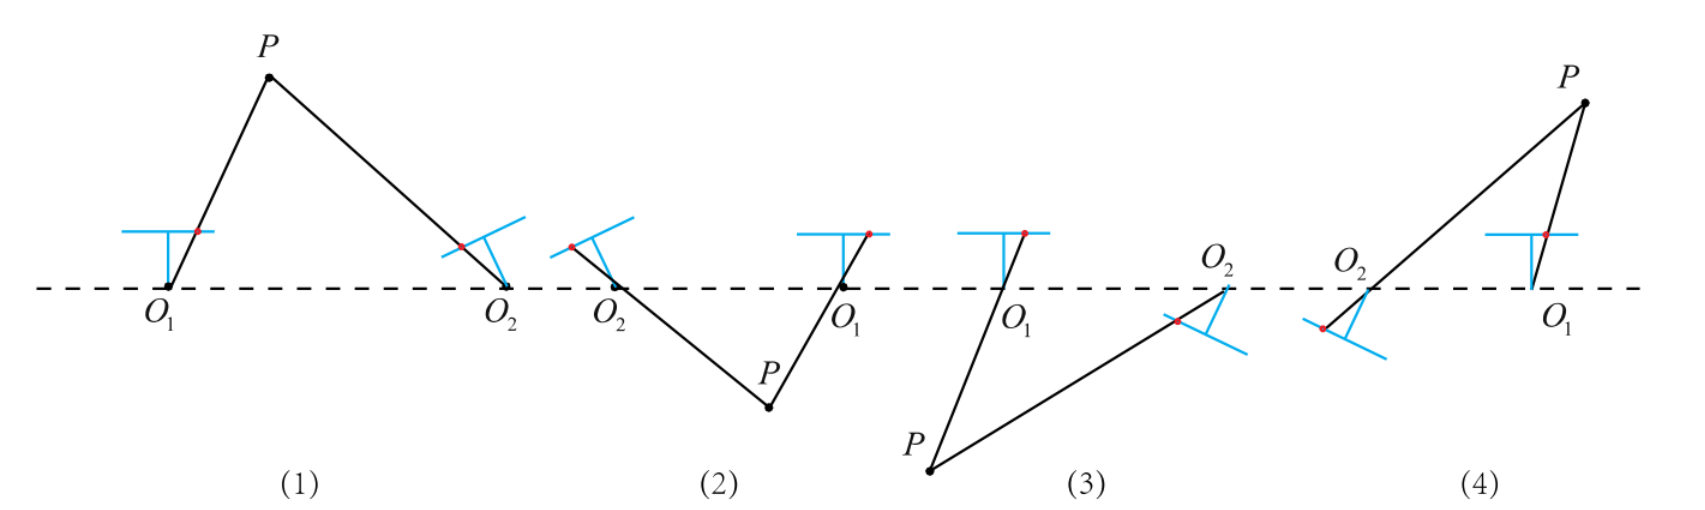
\includegraphics[width=0.7\textwidth]{images/SVD.png}
                                                    \caption{从E分解到R、t存在四种可能性}
                                                \end{figure}
        ==============================\\
        \item \textbf{关于错误匹配与RANSAC优化}
        \begin{enumerate}
            \item \textbf{问题}:当匹配点数量多于8对时,可能包含错误匹配;
            \item \textbf{解决}:采用\textbf{RANSAC(Random Sample Consensus)}算法进行鲁棒估计\footnote{RANSAC通过随机采样与一致性检验,有效剔除误匹配点,提高姿态估计的稳定性。};
            \item 判定内点的准则:(1)点到极线的距离在阈值范围内;(2)图像特征射线与极平面之间的夹角在阈值范围内。
        ==============================\\
        \end{enumerate}
        \end{itemize}
        \end{small}
        \item \textbf{2D-to-2D 对极几何的局限性}
        \begin{itemize}
            \item \textbf{尺度不确定问题}:2D特征不带有深度信息,归一化仅固定比例尺度;
            \item \textbf{初始化需平移运动}:为归一化深度信息需初始化,纯旋转运动,$E$ 退化为\textbf{零矩阵},无法求解 $R$;
        \end{itemize}

        \item \textbf{3D-to-2D:PnP方法(Perspective-n-Point)}
        \begin{itemize}
            \item 用于求解3D点到2D投影点之间的位姿变换;
            \item 给定 $n$ 个\textbf{3D点}及其在图像中的\textbf{投影坐标},求相机位姿;
            \item \textbf{不依赖对极约束},可在\textbf{较少的匹配点}下获得良好的运动估计;
            \item 主要方法:
            \begin{enumerate}
                \item 采用6个点对的\textbf{DLT(Direct Linear Transform)}方法;
                \item 采用3个点对的\textbf{P3P方法(Perspective-3-Point)}——求解投影点a, b, c在相机坐标系下的\textbf{三维坐标},把问题转化为一个\textbf{3D到3D}的位姿估计问题\footnote{通过已知3D点 $A,B,C$ 与其投影点 $a,b,c$ 的对应关系,利用几何三角测量恢复相机位姿。};
                \item 优化后的:\textbf{EPnP, PnP, UPnP};
                \item 构建成最小二乘问题迭代求解:\textbf{Bundle Adjustment(BA)}。
            \end{enumerate}
                                                \begin{figure}[H]
                                                    \centering
                                                    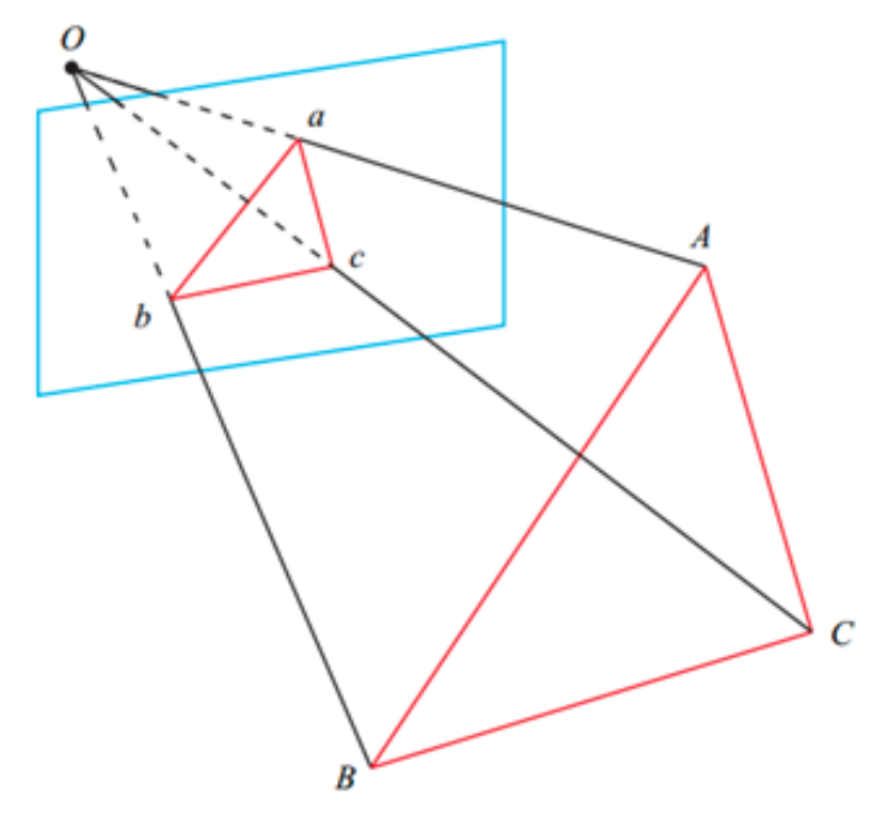
\includegraphics[width=0.4\textwidth]{images/p3p.png}
                                                    \caption{p3p}
                                                \end{figure}
        \end{itemize}
    \end{itemize}

                    \item \textbf{Step4:局部优化} 
                        \begin{itemize}
                            \item \textbf{针对问题}:
                                \begin{enumerate}
                                    \item 特征点对位姿估计存在误差
                                    \item 特征点对存在错误匹配
                                    \item 帧与帧之间的误差不断累积
                                \end{enumerate}
                                    \item \textbf{光束调整法(Bundle Adjustment)}
                                    \begin{itemize}
                                        \item \textbf{原理:}对场景中任意三维点 $X$,由从每个视图所对应的摄像机的光心发射出来并经过图像中 $X$ 对应的像素后的光线,\textbf{都将交于 $X$ 这一点},即对于三维点形成多个光束(bundle)。
    \begin{figure}[H]
        \centering
        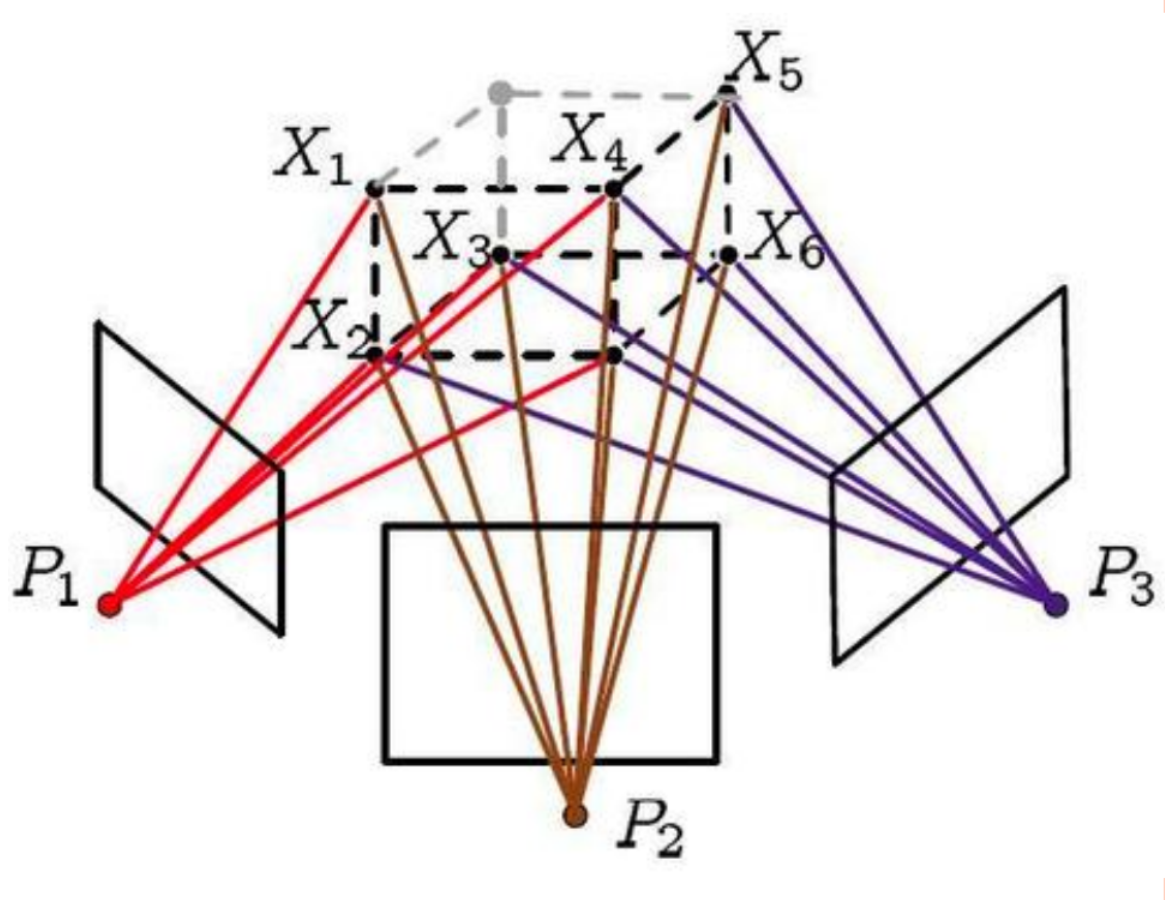
\includegraphics[width=0.34\textwidth]{images/ba.png}
        \caption{光束调整法原理}
    \end{figure}
                                        \begin{small}\kaishu
                                        \item 实际应用中由于噪声等存在,多条光线几乎不可能汇聚于一点,因此在求解过程中,需要不断对待求信息进行调整(adjustment)。
                                        \end{small}
                                        \item \textbf{解决办法}:融合多帧信息,建立\textbf{匹配特征点光束约束},通过\textbf{非线性最优化}求解。
                                        \item \textbf{求解步骤}:
                                        \begin{figure}[H]
                                            \centering
                                            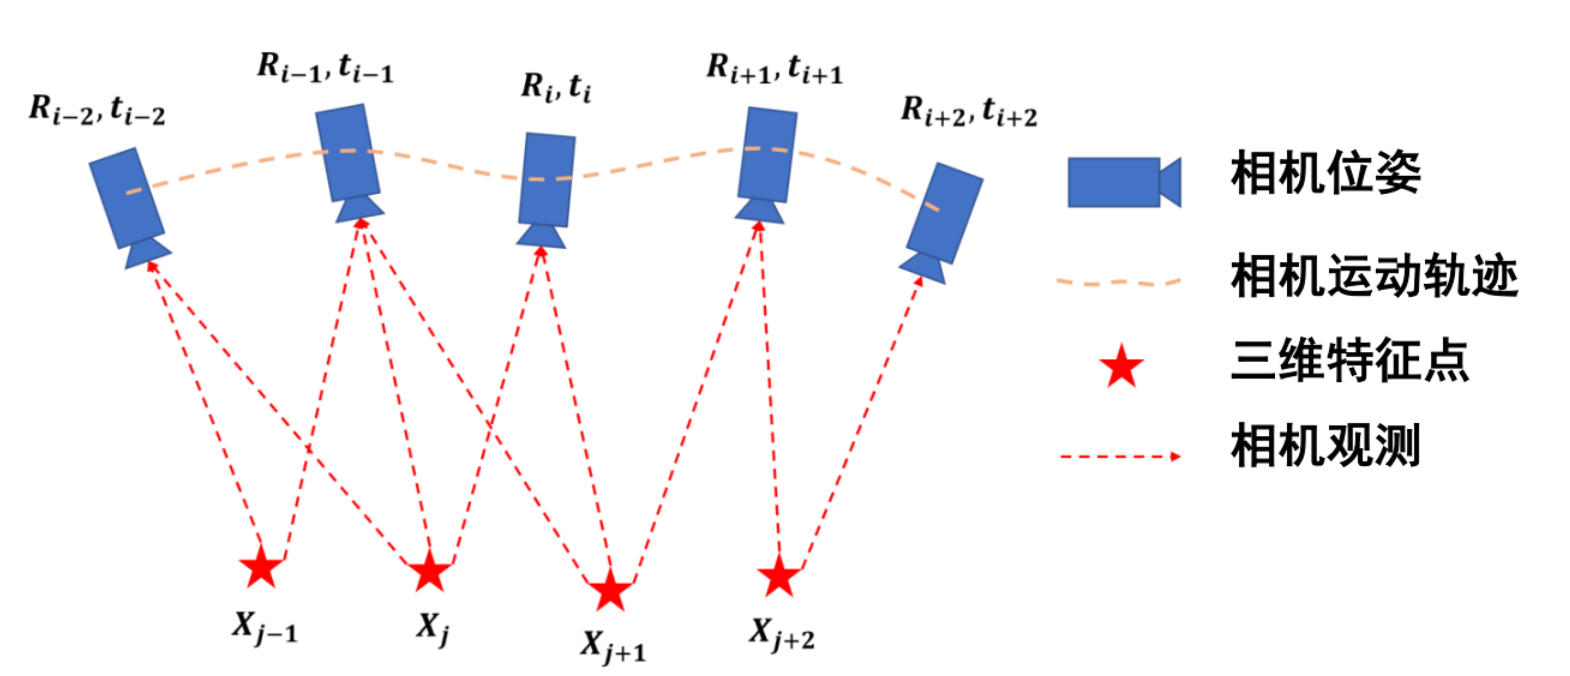
\includegraphics[width=0.7\textwidth]{images/ba2.png}
                                            \caption{光束调整法示例}
                                        \end{figure}
                                        \begin{small}\kaishu
                                        \begin{enumerate}
                                            \item 对于第 $j$ 个三维特征在第 $i$ 时刻图像上的位置:
                                            \[
                                            \tilde{x}_i^j
                                            \]
                                            \item 第 $j$ 个三维特征在第 $i$ 时刻位姿下的图像投影位置:
                                            \[
                                            \pi(R_i, t_i, X_j)
                                            \]
                                            \item 第 $j$ 个三维特征是否出现在第 $i$ 时刻图像:
                                            \[
                                            \kappa_{ij}
                                            \]
                                            \item 光束平移法的优化目标函数为:
                                            \[
                                            \min \sum_{i=1}^{m} \sum_{j=1}^{N} \kappa_{ij} \left\| \tilde{x}_i^j - \pi(R_i, t_i, X_j) \right\|^2
                                            \]
                                        \end{enumerate}
                                        \end{small}
                                    \end{itemize}


                        \end{itemize}
                        \end{itemize}
                \end{enumerate}
        \end{itemize}
\end{enumerate}
\subsection{多信息融合里程估计}
融合多传感器的信息以提高里程估计的性能,主要方法包括EKF、MSCKF等。
\textbf{单一里程计缺陷}:
\begin{itemize}
    \item 轮式里程计:地面不平、轮子打滑等情况下位姿推算不准
    \item IMU:长期位姿估计存在累积误差
    \item 激光:空旷环境、狭长走廊等环境中无法准确估计位姿
    \item 相机:弱纹理环境、图像过曝或过暗时无法估计位姿,单目尺度问题等
\end{itemize}
\end{document}